 \section{Desarrollo} 

Para realizar la demostracion de la funcionalidad de está herramienta,  es necesario realiza los siguientes pasos previos para su aplicación.
\subsection{Instalar herramienta Qlik Sense}

Es necesario para poder realizar esta prueba es necesario saber como instalar esta herramienta , es muy facil e intuitiva los pasos son: 

\begin{itemize}
		\item Ejecutar el instalador como modo administrador, una vez desplegada la ventana. Seleccionaremos la opcion instalar.
\begin{center}
	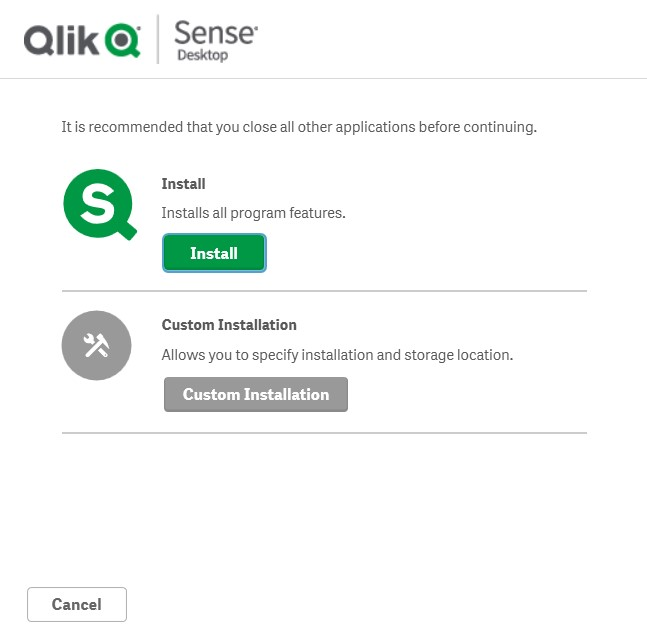
\includegraphics[width=12cm]{./Imagenes/img1} 
\end{center}
		\item Aceptaremos las licencias de la herramienta y daremos siguienta.
\begin{center}
	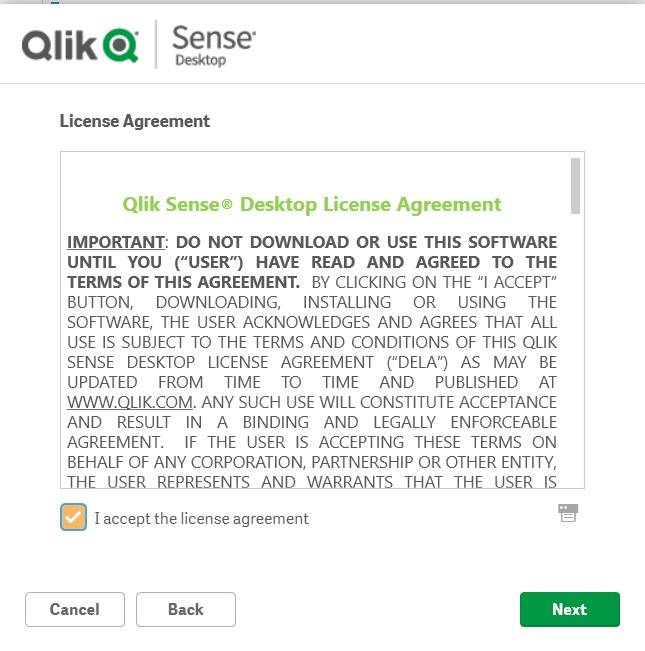
\includegraphics[width=12cm]{./Imagenes/img2} 
\end{center}
		\item Pulsamos el botón «Instalar».
\begin{center}
	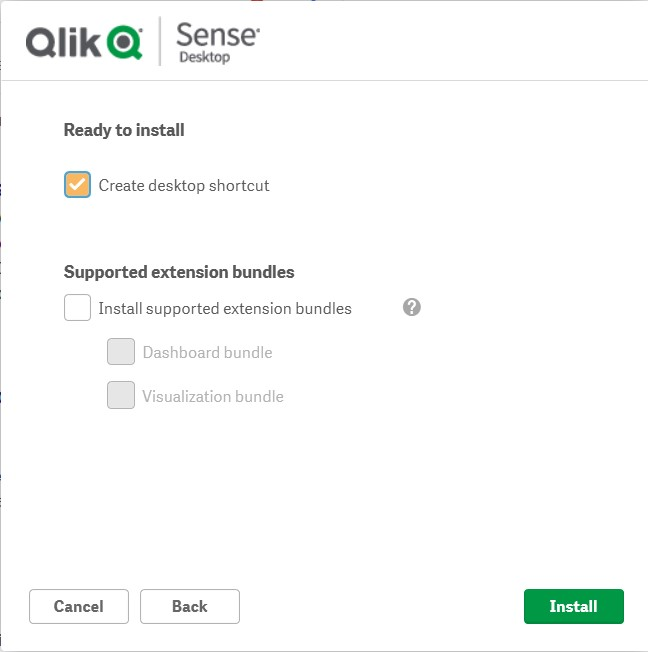
\includegraphics[width=12cm]{./Imagenes/img3} 
\end{center}
\item Esperamos que se complete la instalacion.
\begin{center}
	
\includegraphics[width=12cm]{./Imagenes/img4} 
\end{center}
\item Y tenemos la aplicacion lista para logearnos.
\begin{center}
	
\includegraphics[width=12cm]{./Imagenes/img4} 
\end{center}
\end{itemize}

\subsection{Cargar datos con Qlik Sense}

Lo primero que necesitamos saber para empezar a trabajar con Qlik Sense es saber como cargar nuestra fuente de datos, en este caso vamos a hacerlo paso a paso de una forma bastante detallada. La instalación es verdaderamente sencilla así que pasaremos por alto este paso, solo hay que dar siguiente a todas las ventanas y esperar que la barra de progreso se llene, como es usual en la mayoría de aplicaciones en Windows.
Una vez que tengamos instalado e iniciamos Qlik Sense, lo primero que nos aparecerá es la pantalla de bienvenida:


\begin{center}
	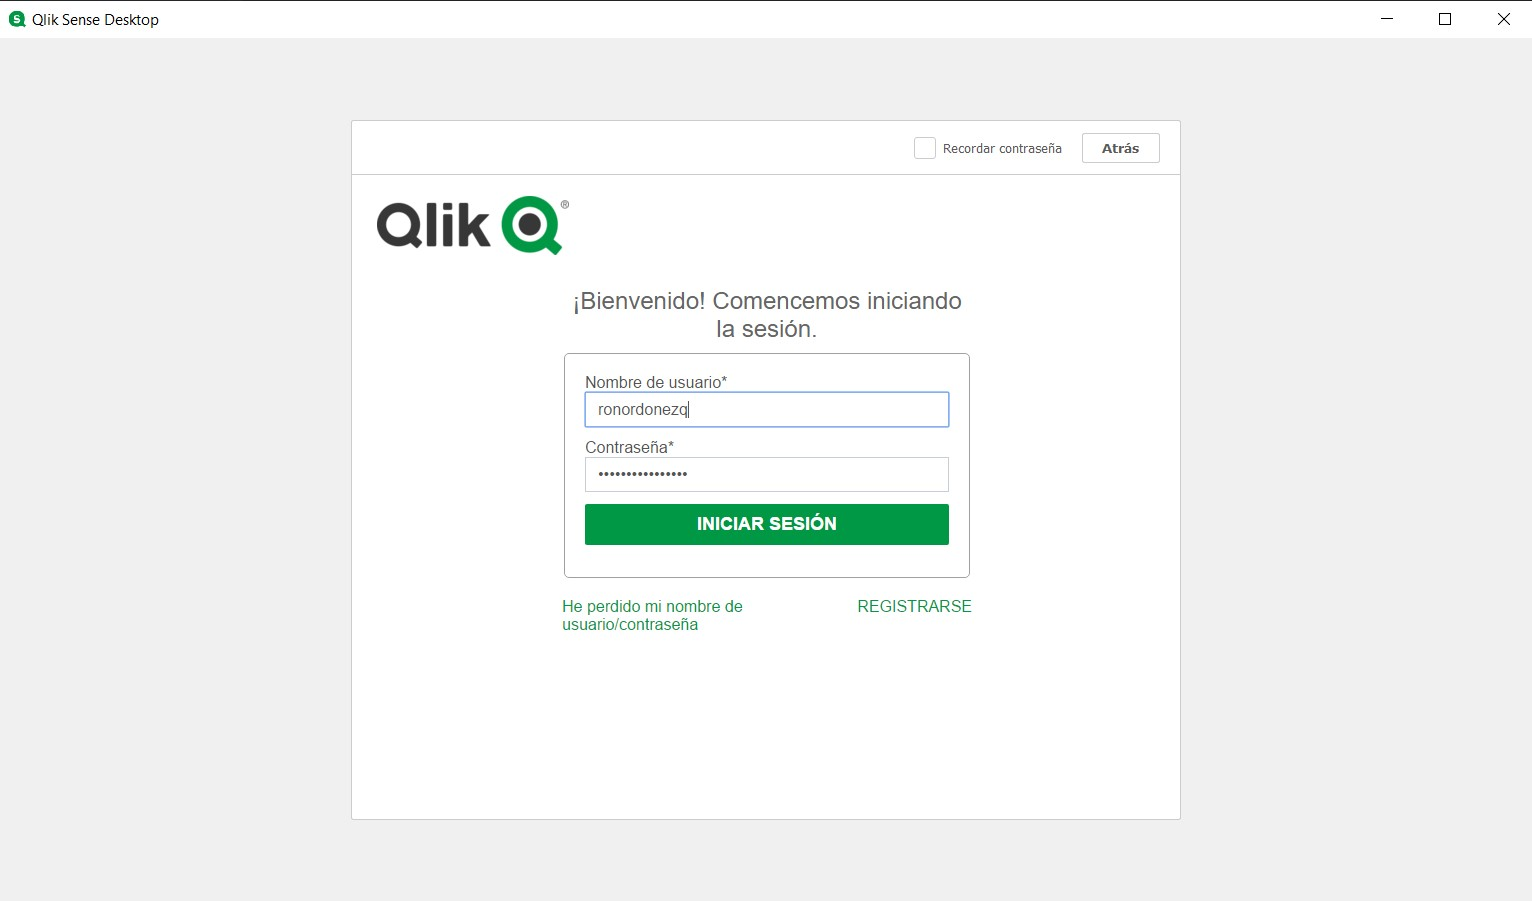
\includegraphics[width=12cm]{./Imagenes/img6} 
\end{center}

Desde aquí deberemos elegir la opción «Crear una nueva App», a continuación se nos pedirá ingresar el nombre para la nueva aplicación que vamos a crear, en mi caso le puse como nombre «TestLoad» y luego pulsar en el botón «Crear».

\begin{center}
	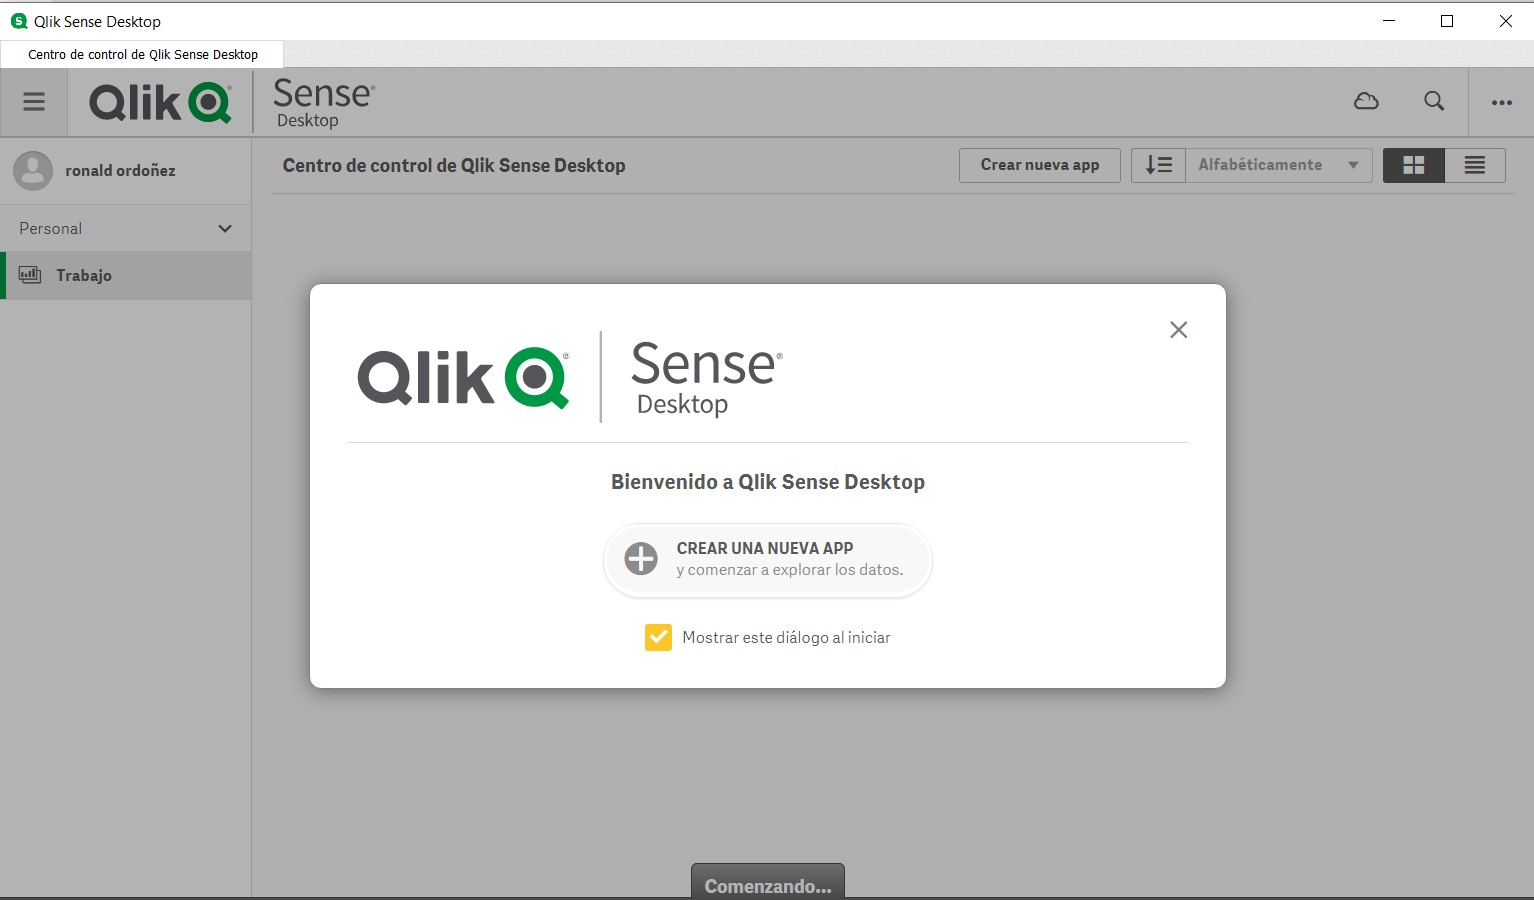
\includegraphics[width=12cm]{./Imagenes/img7} 
\end{center}

En la siguiente vista sólo nos mostrará un mensaje indicando que nuestra app fue creada satisfactoriamente. Ahora pulsar en el botón «Cerrar».
\begin{center}
	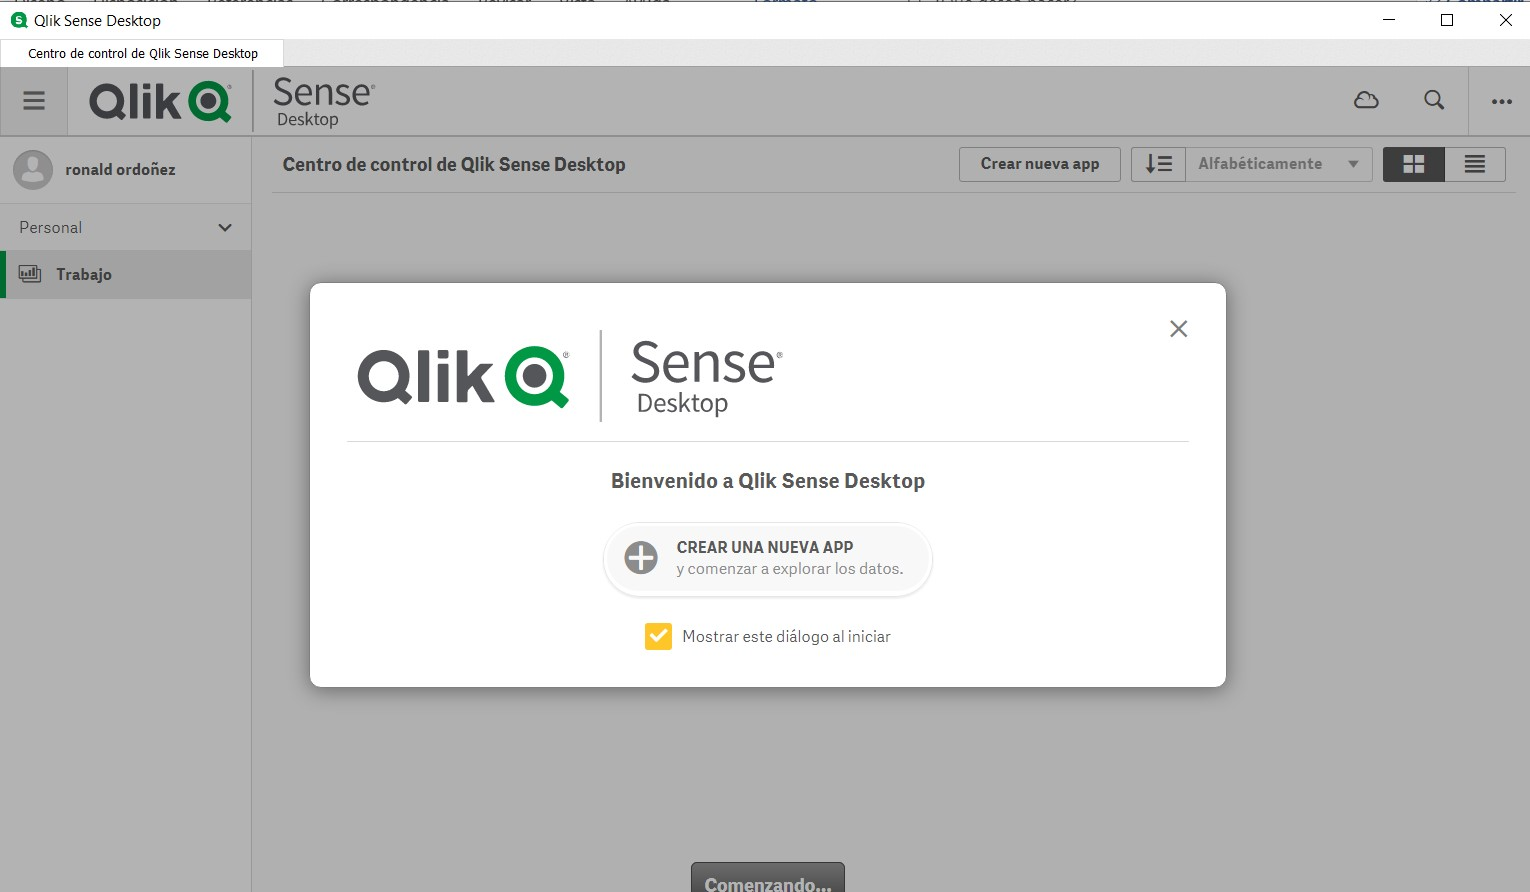
\includegraphics[width=12cm]{./Imagenes/img8} 
\end{center}

A continuación podremos visualizar las dos opciones que nos brinda el Qlik Sense Desktop para poder cargar datos a nuestra aplicación. Estas opciones son:

\begin{itemize}
		\item Carga rápida de datos, con la cual podremos cargar ficheros planos, ya sean estos archivos delimitados por comas (csv, txt, tab, qvo, mem, skv, prn, log), archivos excel (xls, xlw, xlsx, xlsm), archivos HTML (html, htm, php), archivos KML, archivos de registro fijo (fix, dat), archivos de datos QlikView (qvd), archivos de intercambio de datos QlikView (qvx) o archivos XML.
		\item Editor de carga de datos, desde esta opción se tendrá acceso al script de nuestra aplicación, desde donde podremos conectarnos a archivos o bases de datos y realizar el proceso de transformación de datos.
Para este ejemplo elegir la primera opción «Carga rápida de datos».
\end{itemize}


\begin{center}
	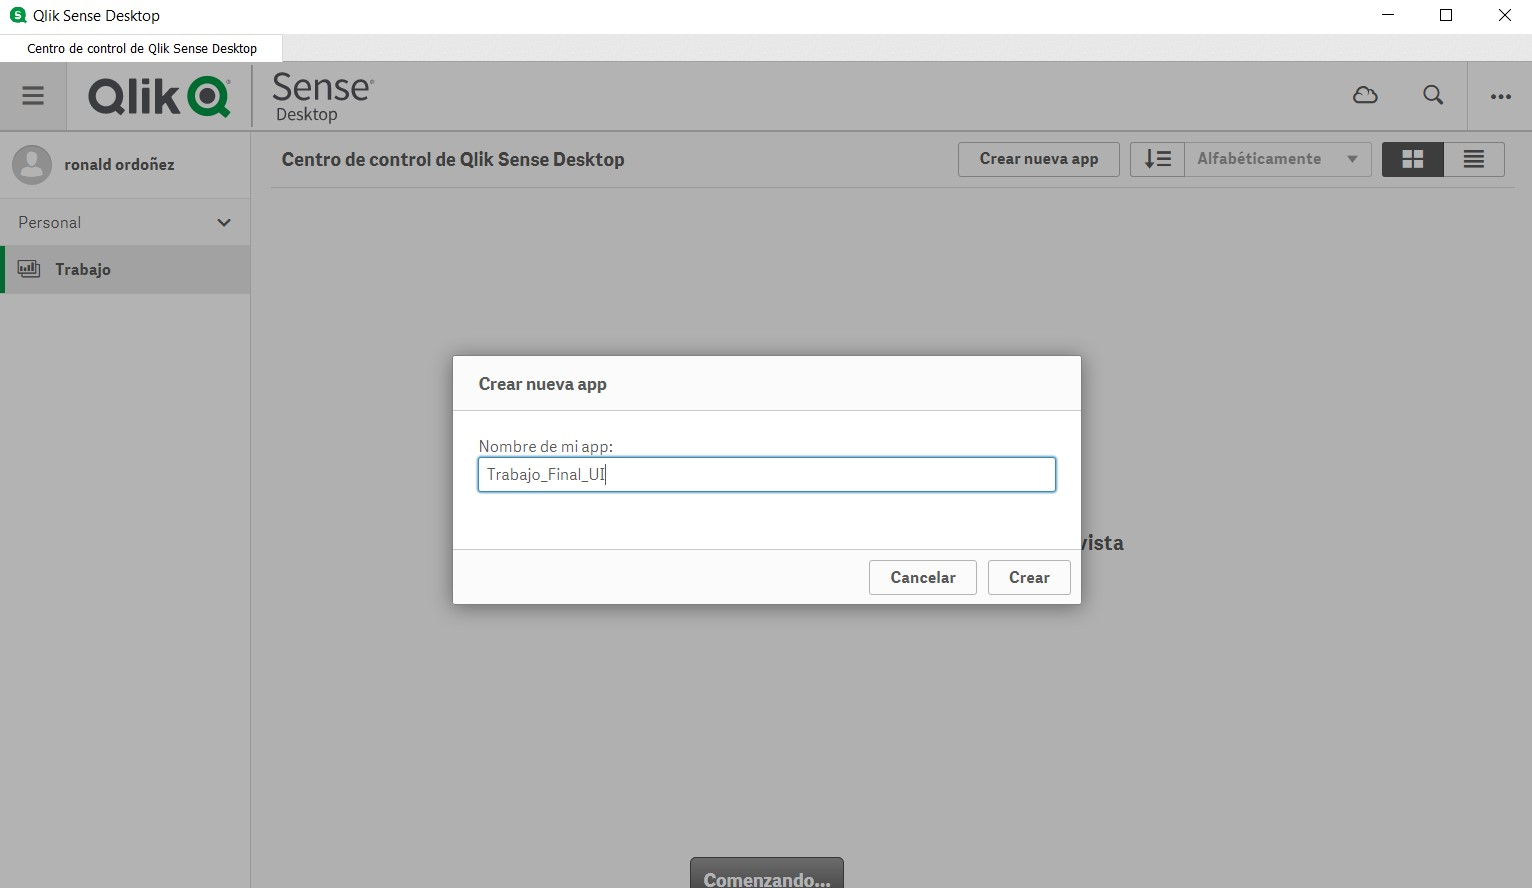
\includegraphics[width=12cm]{./Imagenes/img9} 
\end{center}


Ahora el asistente pedirá ubicar el archivo que se desea cargar, en mi caso voy a tomar un Qvd el cual ya fue procesado en un proyecto anterior.
\begin{center}
	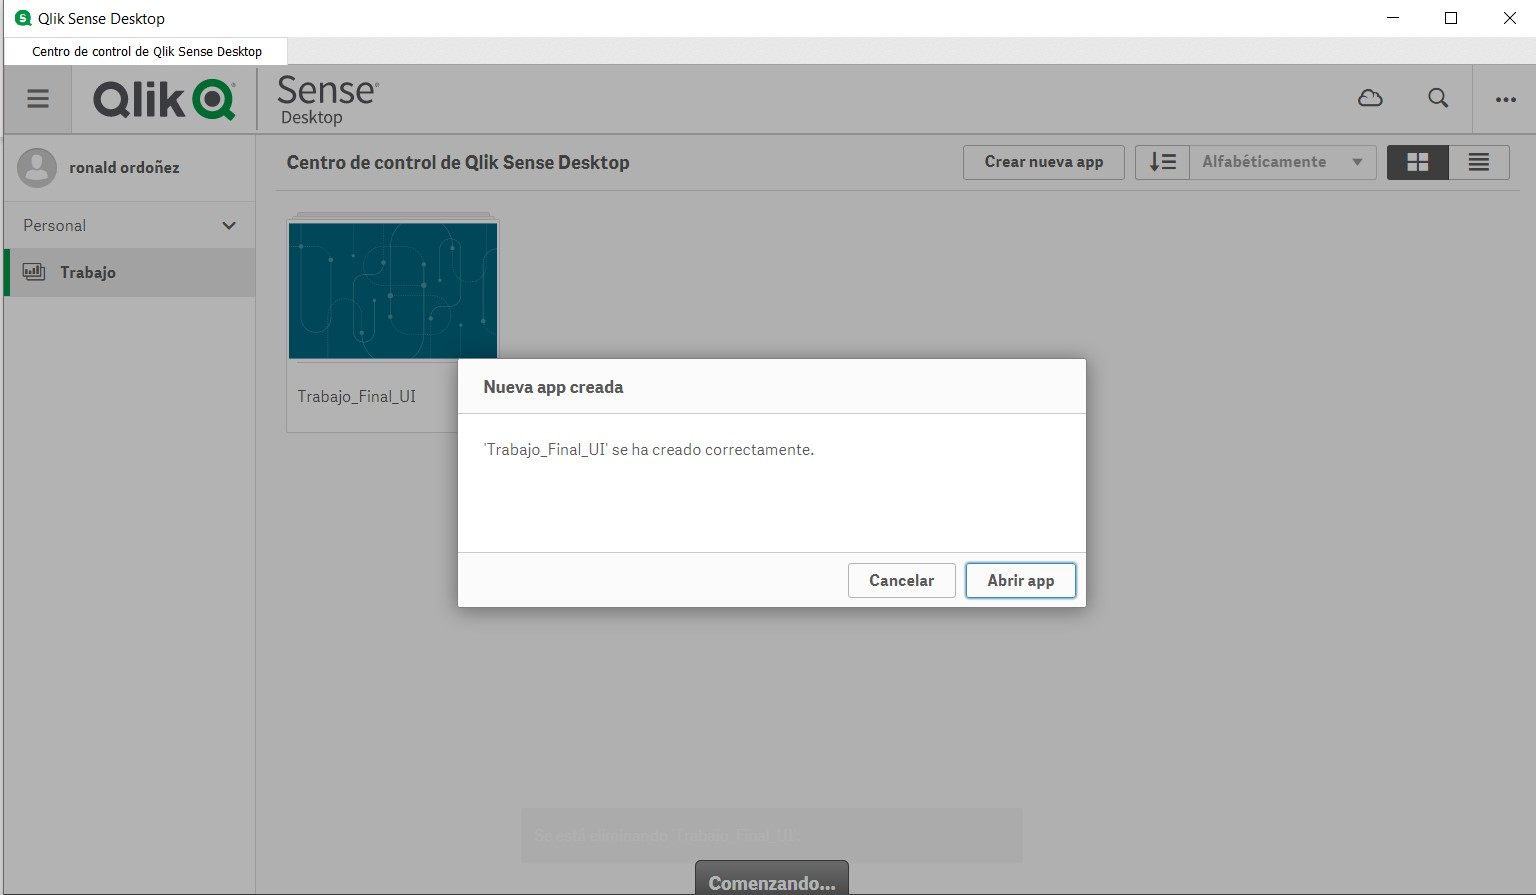
\includegraphics[width=12cm]{./Imagenes/img10} 
\end{center}

En la siguiente vista, se podrá visualizar una muestra de los datos a cargar y los nombres de sus campos.
Por defecto aparece marcado el check que dice «Seleccionar todos los campos», con lo cual se cargará todas las columnas a nuestra aplicación. En caso no se desee cargar todo, se puede marcar/desmarcar el check que tiene cada columna y de esta forma dejar solo las que se necesita.
Además del buscador que nos permitirá ubicar rápidamente los campos que necesitamos, si se hace doble clic en el título de una columna, exactamente sobre el nombre, se activará un mini editor desde donde se podrá renombrar la columna que deseemos.
Una vez seleccionados y renombrados los campos que deseemos, pulsar en el botón «Cargar datos» que se encuentra en la parte inferior derecha.

\begin{center}
	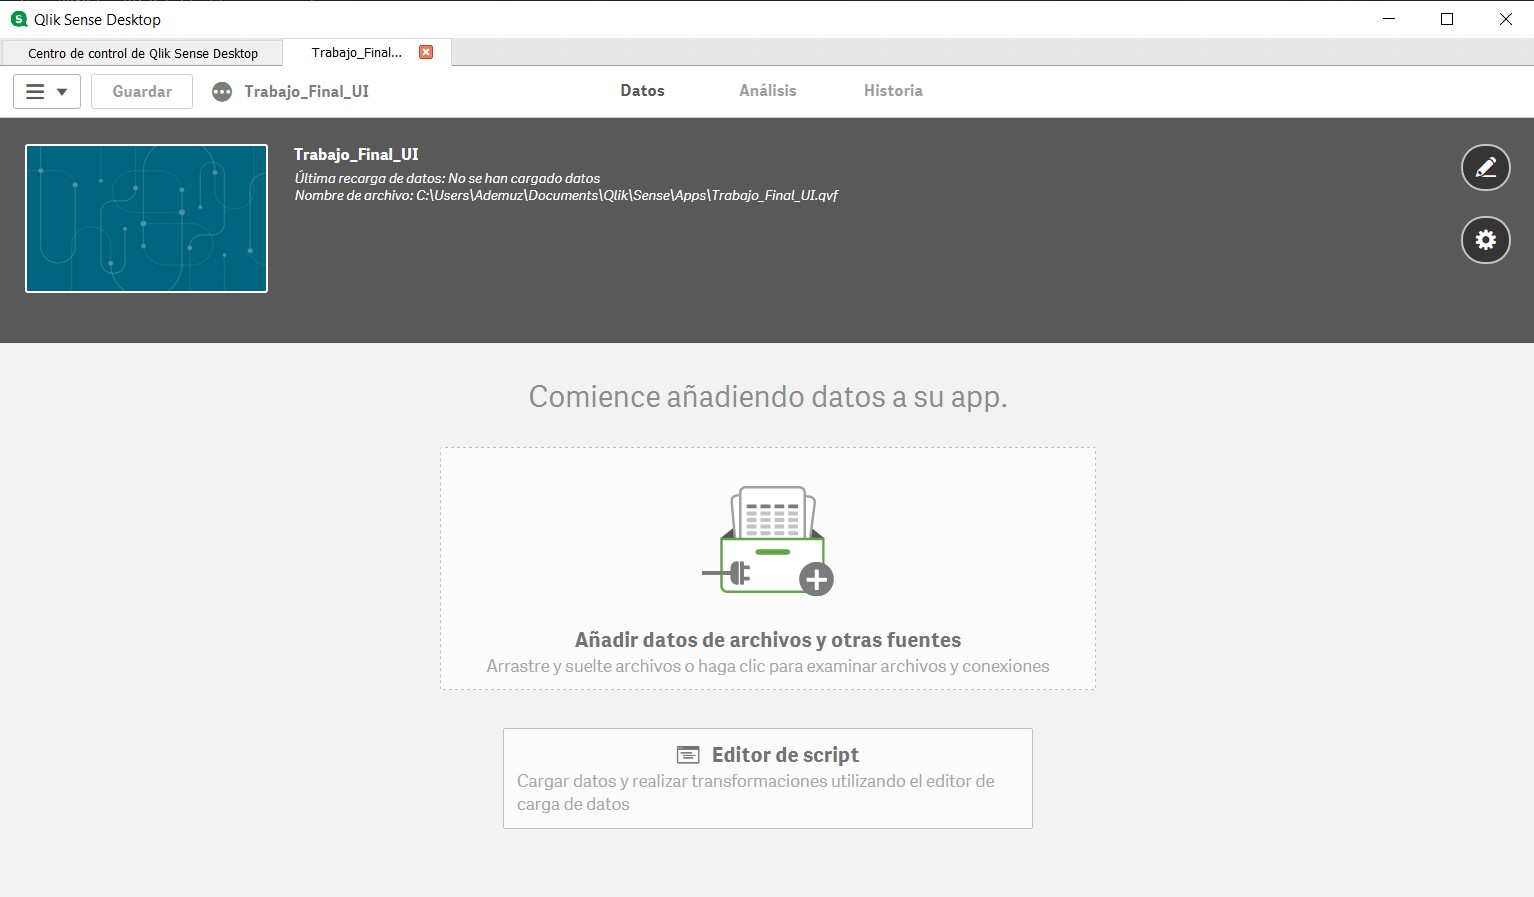
\includegraphics[width=12cm]{./Imagenes/img11} 
\end{center}

La carga como es usual cuando trabajamos con archivos Qvds será bastante rápida y una vez terminada nos aparecerá la siguiente ventana indicando el tiempo que ha tomado realizar la carga, en esta ventana solo pulsar «Cerrar» para poder.

\begin{center}
	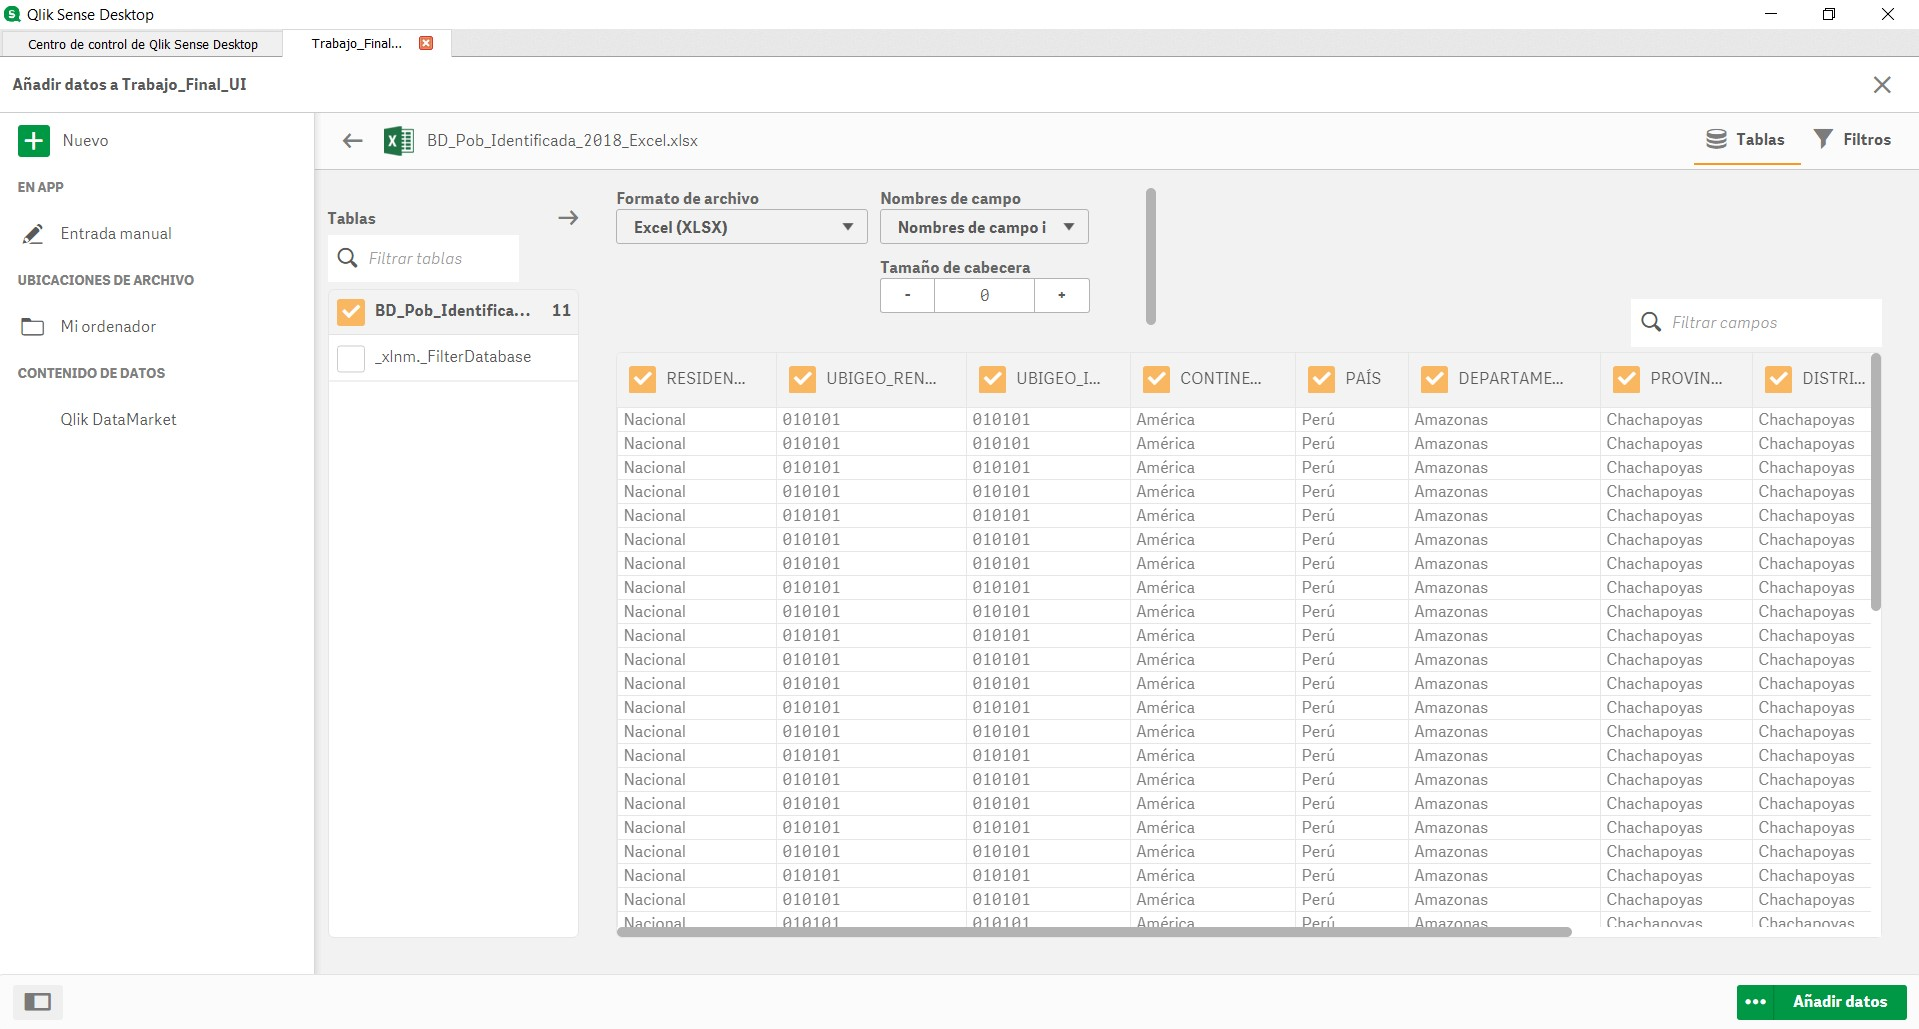
\includegraphics[width=12cm]{./Imagenes/img12} 
\end{center}

Luego de esto estaremos en nuestra aplicación como tal, vamos a revisar las opciones que tenemos disponibles en los menús, en el primero se ve como deshabilitado el botón de «Vista general de app», ya que es justo donde nos encontramos.
